\documentclass[10pt,a4paper]{article}
\usepackage[a4paper,left=15mm,right=15mm,top=16mm,bottom=18mm]{geometry}

% -----------------------------------------------------------------------------
% Fonts & Localization (XeLaTeX)
% -----------------------------------------------------------------------------
\usepackage{fontspec}
\usepackage{xunicode}
\usepackage{xltxtra}
\defaultfontfeatures{Mapping=tex-text}

\setmainfont{Bai Jamjuree}[
  UprightFont=* Regular,
  BoldFont=* SemiBold,
  ItalicFont=* Italic,
  BoldItalicFont=* SemiBold Italic
]

% -----------------------------------------------------------------------------
% Essential Packages
% -----------------------------------------------------------------------------
\usepackage{amsmath,amssymb,amsfonts}
\usepackage{booktabs}
\usepackage{tabularx}
\usepackage{colortbl}
\usepackage{xcolor}
\usepackage{graphicx}
\usepackage{enumitem}
\usepackage{fancyhdr}
\usepackage{hyperref}
\usepackage{caption}
\usepackage{tcolorbox}
\tcbuselibrary{skins,breakable}

% -----------------------------------------------------------------------------
% Header & Footer Settings
% -----------------------------------------------------------------------------
\setlength{\headheight}{14pt}
\setlength{\headsep}{10pt}
\pagestyle{fancy}
\fancyhf{}
\renewcommand{\headrulewidth}{0.5pt}
\renewcommand{\footrulewidth}{0.4pt}
\fancyhead[L]{\small \textbf{\textcolor{primary}{NEXVIA AEGIS: Autonomous Physical AI Research Program}}}
\fancyhead[R]{\small \textcolor{darkgray}{Milestone V9-M17 \textbar\ Team Roadmap}}
\fancyfoot[L]{\footnotesize \textcolor{darkgray}{เอกสารทางการ: โครงสร้างงานวิจัย การทดลอง และการแบ่งงาน 3 คน}}
\fancyfoot[R]{\footnotesize \textbf{หน้า \thepage}}

% -----------------------------------------------------------------------------
% Color Palette: Academic Executive Deep Blue / Slate
% -----------------------------------------------------------------------------
\definecolor{primary}{RGB}{15, 34, 64}        % Deep Navy
\definecolor{secondary}{RGB}{28, 78, 128}     % Slate Blue
\definecolor{accent}{RGB}{180, 83, 9}         % Warm Amber / Bronze
\definecolor{highlight}{RGB}{13, 148, 136}    % Teal
\definecolor{lightbg}{RGB}{248, 250, 252}     % Crisp Light Slate
\definecolor{cardborder}{RGB}{203, 213, 225}  % Slate Border
\definecolor{darkgray}{RGB}{51, 65, 85}

\hypersetup{
  colorlinks=true,
  linkcolor=secondary,
  filecolor=secondary,
  urlcolor=secondary,
  citecolor=secondary
}

% -----------------------------------------------------------------------------
% Custom Callout Boxes
% -----------------------------------------------------------------------------
\newtcolorbox{anchorbox}{
  colback=secondary!5!white,
  colframe=secondary,
  arc=2.5mm,
  boxrule=1pt,
  left=8pt,
  right=8pt,
  top=6pt,
  bottom=6pt,
  title=\textbf{\normalsize สมอวิจัยและแกนแนวคิดหลักของโครงการ (Core Research Anchor)},
  fonttitle=\bfseries\color{white},
  colbacktitle=secondary
}

\newtcolorbox{infobox}[1]{
  colback=lightbg,
  colframe=cardborder,
  arc=2mm,
  boxrule=0.7pt,
  left=8pt,
  right=8pt,
  top=5pt,
  bottom=5pt,
  title=\textbf{\normalsize #1},
  fonttitle=\bfseries\color{primary},
  colbacktitle=cardborder!35!white
}

\newtcolorbox{rolebox}[2]{
  colback=#2!3!white,
  colframe=#2,
  arc=2.5mm,
  boxrule=0.9pt,
  left=8pt,
  right=8pt,
  top=5pt,
  bottom=5pt,
  title=\textbf{\normalsize #1},
  fonttitle=\bfseries\color{white},
  colbacktitle=#2
}

\begin{document}
\enlargethispage{2\baselineskip}

% =============================================================================
% PAGE 1: TITLE & SECTION 1: RESEARCH PROBLEM & CORE ANCHOR
% =============================================================================
\begin{center}
  {\LARGE \textbf{\textcolor{primary}{NEXVIA AEGIS: AUTONOMOUS PHYSICAL AI}}}\\[3pt]
  {\large \textbf{\textcolor{secondary}{รายงานสรุปรายละเอียดงานวิจัย กรอบทฤษฎี และโครงสร้างการแบ่งงานทีม 3 คน}}}\\[2pt]
  {\small \textit{Master Research Blueprint, Theoretical Foundations, 17-Phase Progress \& Team Work Breakdown}}
  \vspace{4pt}

  \footnotesize
  \begin{tabular}{rlrl}
    \textbf{รหัสเอกสาร:} & \texttt{AEGIS-RES-TEAM-2026-11} & \textbf{วันที่อัปเดต:} & พฤศจิกายน 2026 \\
    \textbf{สถานะโครงการ:} & Milestone V9-M17 Certified & \textbf{ชุดทดสอบระบบ:} & ผ่าน 872 / 872 Tests (100\%) \\
    \textbf{ผู้เขียนหลัก / หัวหน้าทีมวิจัย:} & นายเฉลิมศักดิ์ (Lead Researcher \& Architect) & \textbf{Git Repository:} & \texttt{Chalermsak1/nexvia-aegis} \\
  \end{tabular}
\end{center}

\vspace{1pt}
\section*{\textcolor{secondary}{\large 1. โจทย์งานวิจัยและแกนแนวคิดหลัก (Research Problem \& Core Anchor)}}
\vspace{-4pt}

\begin{anchorbox}
  {\small \textbf{``NEXVIA AEGIS is a risk-aware autonomy framework designed to enable intelligent systems to verify the reliability of their observations and decisions before taking action, allowing them to act when sufficiently safe and abstain when uncertainty or risk is too high.''}}
  \vspace{2pt}
  \tcblower
  \footnotesize
  \textbf{ความหมายเชิงปฏิบัติการ (Operational Translation):}
  NEXVIA AEGIS คือกรอบการทำงานอัตโนมัติตระหนักรู้ความเสี่ยงสำหรับระบบปัญญาประดิษฐ์กายภาพ (Physical AI) และหุ่นยนต์ เพื่อให้ระบบสามารถ \textbf{ตรวจสอบความน่าเชื่อถือของการสังเกต (Observations) และการตัดสินใจ (Decisions) ของตนเองก่อนลงมือกระทำจริง} โดยระบบจะได้รับอนุญาตให้ขับเคลื่อนกระทำการเมื่อมีความปลอดภัยเพียงพอ และสามารถ \textbf{สละสิทธิ์การตัดสินใจ (Abstain) ยุติการกระทำและนำยานยนต์เข้าสู่สถานะหยุดนิ่งสนิท} เมื่อความไม่แน่นอนหรือความเสี่ยงสูงเกินกว่าขอบเขตความปลอดภัย
\end{anchorbox}

\vspace{2pt}
\subsection*{\normalsize 1.1 โจทย์ปัญหาทางวิชาการที่งานวิจัยนี้ต้องการแก้ไข (Core Research Problems)}
\vspace{-3pt}
ในระบบขับขี่อัตโนมัติ (AV) และหุ่นยนต์ทางอากาศ (UAV) ทั่วโลก ปัจจุบันเผชิญกับ \textbf{4 คอขวดใหญ่ ที่ไม่เคยมีระบบใด ตอบโจทย์ได้ครบ}:
\begin{enumerate}[leftmargin=14pt, itemsep=1pt, topsep=1pt, parsep=0pt]
  \item \textbf{ปัญหาความมั่นใจเกินจริง และการกระทำแบบตาบอด (Overconfidence \& Blind Execution):} หุ่นยนต์ทั่วไป พยายามขับเคลื่อน เข้าหาเป้าหมาย ตลอดเวลา แม้เซนเซอร์ เกิดความผิดปกติ เช่น เลนส์เปื้อน, แสงสะท้อนจ้า (Glare), หมอกควัน, สัญญาณ LiDAR หลุด (Blackout) ส่งผลให้ ขับเคลื่อนด้วย สภาวะที่คลาดเคลื่อน จนพุ่งชน สิ่งกีดขวาง
  \item \textbf{ปัญหาการแช่แข็งที่จุดสมมาตร (The Freezing Dilemma at Saddle Points):} ระบบควบคุม ความปลอดภัย ดั้งเดิม (เช่น Passive CBF) เมื่อพบสิ่งกีดขวาง ขวางแนวเป้าหมาย แรงดึงดูด กับแรงต้าน จะหักล้างกัน เป็นศูนย์ ($\mathbf{u} \to \mathbf{0}$) ทำให้หุ่นยนต์ จอดค้างเติ่ง (Passive Freeze) ทั้งที่มี ช่องว่างเปิด ด้านข้าง
  \item \textbf{ความคลุมเครือเชิงภววิทยา (Saddle Point vs. Impasse Ambiguity):} เมื่อหยุดนิ่ง หุ่นยนต์ ไม่สามารถ แยกแยะได้ ด้วยการอยู่เฉยๆ ว่า ตรงหน้านั้น เป็น \textit{"สิ่งกีดขวาง ที่เบี่ยงหลบได้"} หรือเป็น \textit{"ซอยตัน ที่ไม่มีทางไป (Cul-de-Sac)"}
  \item \textbf{การอ้างว่าถึงเป้าหมายแบบเท็จ และการขาดการสละสิทธิ์ ทางกายภาพ (False Arrival \& Lack of Grounded Abstention):} หุ่นยนต์จำนวนมาก เพียงแค่เหยียบพิกัด ก็ประกาศว่าสำเร็จ ทั้งที่โมเมนตัม ยังพุ่งชน กำแพงด้านหลัง (ขาด Physical Dwell Verification) และเมื่อ หมดทางไป ก็ไม่สามารถ ส่งสัญญาณ สละสิทธิ์ ที่มีหลักฐาน รองรับได้
\end{enumerate}

\vspace{2pt}
\subsection*{\normalsize 1.2 เสาหลักทางทฤษฎีของ NEXVIA AEGIS (Theoretical Pillars)}
\vspace{-3pt}
\begin{itemize}[leftmargin=14pt, itemsep=1pt, topsep=1pt, parsep=0pt]
  \item \textbf{Information-Theoretic Observability Gate:} ตรวจสอบ ค่าความแปรปรวน ของการประมาณ สถานะ ($\sigma_{p,\max} \le 0.25\,$m, $\sigma_{v,\max} \le 0.35\,$m/s) หากเซนเซอร์ Blackout จน Covariance พองตัว ระบบจะสั่ง ปฏิเสธคำสั่ง และเข้าสู่ Safe Abstain เบรกหยุดนิ่ง ทันที
  \item \textbf{Robust Tube-CLBF \& Micro-QP Optimization:} ผสาน Control Barrier Functions (CBF) ขยายระยะเผื่อ ความปลอดภัย ตามความไม่แน่นอน ($\kappa_\delta \sqrt{\nabla h^T \boldsymbol{\Sigma} \nabla h}$) ร่วมกับ Control Lyapunov Functions (CLF) แก้สมการด้วย Micro-QP ความเร็วสูง ($<0.2\,$ms, Feasible 100\%)
  \item \textbf{Anytime-Valid Ville's Supermartingale Risk Control:} ใช้ทฤษฎี Martingale ของ Ville ตรวจจับการแอบดึง Slack ความปลอดภัย สะสมเกินเกณฑ์ ความเสี่ยง ($p \le 10^{-3}$) หากพบการฝ่าฝืน จะตัดระบบ เข้าสู่ Fail-Closed Active Stop ทันที
  \item \textbf{Bounded Active Probing POMDP:} เมื่อยานยนต์ ชะลอตัวนิ่ง ระบบจะสร้าง แรงเร่งสำรวจ ขนาดจำกัด ในแนวสัมผัส ภายใต้ เกราะคุ้มกัน Tube-CBF (0.0\% Collision) เพื่อสำรวจ หาช่องเปิด หรือหากพิสูจน์ ได้ว่าปิดตาย ครบทุกทิศทาง จะส่งมอบ การสละสิทธิ์ ทางกายภาพ อย่างสมบูรณ์
  \item \textbf{Terminal Physical Stillness \& Active Dwell Verification:} บังคับใช้ การตรวจวัด พลังงานจลน์จริง $E_k \le 0.005\,$J และการเบรก แบบ Deadbeat Damping ติดต่อกัน $N_{\text{dwell}} \ge 15$ สเต็ป เพื่อยืนยันว่า ยานยนต์ หยุดนิ่งสนิทจริง
\end{itemize}

\newpage

% =============================================================================
% PAGE 2: SECTION 2: 17 PHASES OVERVIEW TABLE
% =============================================================================
\section*{\textcolor{secondary}{\large 2. รายละเอียดงานทั้งหมดที่ทำมา (Chronological Milestone Overview: Phases 1 to 17)}}
\vspace{-4pt}

โครงการ NEXVIA AEGIS ได้รับการพัฒนา วิจัย และทดสอบอย่างต่อเนื่องผ่าน 17 เฟสหลัก ครอบคลุมตั้งแต่การตัดสินใจเชิงทฤษฎี หุ่นยนต์ทางอากาศ 6-DOF ขบวนรถยนต์ภาคพื้นดิน จนถึงสถาปัตยกรรม Tube-CLBF และ Active Probing:

\vspace{3pt}
\subsection*{\normalsize 2.1 เฟส 1--9: รากฐานทฤษฎีความปลอดภัยและวิวัฒนาการหุ่นยนต์เดี่ยว (Foundations \& Single-Agent Evolution)}
\vspace{-3pt}

\begin{center}
\footnotesize
\begin{tabularx}{\textwidth}{>{\centering\arraybackslash}p{0.6cm} >{\raggedright\arraybackslash}p{3.2cm} >{\raggedright\arraybackslash}X >{\raggedright\arraybackslash}p{4.7cm}}
\toprule
\textbf{Phase} & \textbf{ชื่อเฟสและหัวข้อหลัก} & \textbf{สถาปัตยกรรมและอัลกอริทึมสำคัญ} & \textbf{ผลลัพธ์เชิงประจักษ์ (Key Metrics)} \\
\midrule
\textbf{1} & Trustworthy Decision-Making & Ville Supermartingale Sequential Risk Control, Matched Benchmark 1,800 episodes & False Alarm UCB $\le 0.0034$, Active Probing gain +39.17\% TSR \\
\textbf{2} & Continuous 3D Physical AI & Aegis3DAwareController, 3D CBF Safe Braking & TSR 80.0\% vs 13.3\% (naive), Obstacle Collision 0.0\% \\
\textbf{3} & Decentralized Swarm Resilience & Colluding Byzantine Spoofing ($F=2$), Packet Loss 25\%, Trimmed BRMC & Localization Error ลดลง 97.8\%, Swarm Collision 0.0\% \\
\textbf{4} & 6-DOF Quadrotor Dynamics & SE(3) Rigid-Body MuJoCo, Motor Lag $\tau_m=35$ms, Reciprocal Underactuated HOCBF & จำกัดมุมเอียง $\theta \le 35^\circ$, ป้องกัน Rotor Saturation สมบูรณ์ \\
\textbf{5} & Deep Aerodynamics & Ground Effect ($T_{\text{IGE}}$), Gyroscopic Precession, 4S LiPo Voltage Sag Dynamic Thrust & ทนต่อลมดูดและแรงบิดหมุนควง, Zero Thrust Drop Crashes \\
\textbf{6} & Safe Reinforcement Learning & Actor-Critic (PPO) ผสาน HOCBF Action Shield หลบหลีกสิ่งกีดขวางแบบไดนามิก & ชน 0 ครั้งระหว่างเทรน (vs 8 crashes), ลด Barrier Intervention ลง 21.0\% \\
\textbf{7} & Active Vision \& LiDAR SLAM & Simulated Depth Camera, Raycast Occlusion, 7-state UKF Covariance Inflation & ชน 0.0\% ในช่องแคบ (vs 100\% blind), รักษาระยะปลอดภัย $+0.271\,$m \\
\textbf{8} & Sim2Real Hardware Bridge & ROS 2 Humble node, MAVLink 200Hz, Latency Extrapolation, Safety Watchdog & ทนต่อ Jitter 15ms \& Packet Drop 3\%, Failsafe Hover ใน 60ms \\
\textbf{9} & NMPC-CBF Lookahead & 15-step ($0.75\,$s) Receding Horizon D-CBF, Jerk Minimization, Real-Time sub-50ms & ขจัด Altitude Ballooning และการเบรกกระตุก, Fallback Shield 100\% \\
\bottomrule
\end{tabularx}
\end{center}

\vspace{3pt}
\subsection*{\normalsize 2.2 เฟส 10--17: ระบบทีมพาหนะไฮบริด, Robust Tube-CLBF และ Bounded Active Probing}
\vspace{-3pt}

\begin{center}
\footnotesize
\begin{tabularx}{\textwidth}{>{\centering\arraybackslash}p{0.6cm} >{\raggedright\arraybackslash}p{3.2cm} >{\raggedright\arraybackslash}X >{\raggedright\arraybackslash}p{4.7cm}}
\toprule
\textbf{Phase} & \textbf{ชื่อเฟสและหัวข้อหลัก} & \textbf{สถาปัตยกรรมและอัลกอริทึมสำคัญ} & \textbf{ผลลัพธ์เชิงประจักษ์ (Key Metrics)} \\
\midrule
\textbf{10} & Ground AV \& Platooning Stack & Dynamic Bicycle Model, Pacejka Magic Formula, Frenet HOCBF, V2X Spoof Defense & Kamm's Friction Anti-Skid บนถนน $\mu=0.35$, ดักจับ Phantom Brake ใน 540ms \\
\textbf{11} & Air-Ground Heterogeneous Team & Eye-in-the-Sky Quadrotor Scout บินนำ $65\,$m, V2A Wireless Telemetry, Lookahead Stop & เตือนลื่นล่วงหน้า $150\,$m, Stopping Margin $+10.21\,$m ก่อนถึงจุดอันตราย \\
\textbf{12} & Multi-Vehicle Scout Handover & Dual Scout Handover State Machine, V2V Multi-Hop CBF, String Stability & $\|G(j\omega)\|_\infty = 1.000$ ไม่มีคลื่นเบรกสะท้อน, ป้องกันการชนท้าย 100\% \\
\textbf{13} & Robust Tube-CLBF & ปิด 4 Core Bottlenecks: Conservatism, Speed Gate, Physical Dwell, Micro-QP & Micro-QP รัน $<0.2\,$ms, Feasible 100\%, Stillness $E_k \le 0.005\,$J \\
\textbf{14} & Delay Compensation Benchmark & Exact ZOH Forward Projection ($\tau \in [15, 60]\,$ms) บน 100 โลกใหม่ (Seeds 2000+) & Naive ชน 100/100, AEGIS ชน 0/100 (0.0\% Collision Rate), Selective Risk 0\% \\
\textbf{15} & Parametric Mass Invariance & Worst-Case Authority Derating $\beta_{\min} \approx 0.769$ รับมือ $\Delta_m = \pm 30\%$ (Seeds 3000+) & เพิ่มระยะห่างปลอดภัยเมื่อบรรทุกหนักเป็น 1.653 m (+21.5 cm), ชน 0.0\% \\
\textbf{16} & Sensor Blackout Gate & Observability Gate ($\sigma_p \le 0.25\,$m, $\sigma_v \le 0.35\,$m/s), Zero Truth Leakage (Seeds 4000+) & ป้องกันการชนในความมืด 100.0\% (66/66), รักษาระยะห่างเฉลี่ยใน Blackout 2.054 m \\
\textbf{17} & Bounded Active Probing & Tangential Micro-Probing คลี่คลาย Saddle Points และ Cul-de-Sac (Seeds 5000+) & ความสำเร็จภาพรวมพุ่งสู่ \textbf{93.0\%} (vs 60\% passive), สละสิทธิ์ซอยตัน 90.9\% \\
\bottomrule
\end{tabularx}
\end{center}

\newpage

% =============================================================================
% PAGE 3: BENCHMARK VISUALS 1 & 2
% =============================================================================
\section*{\textcolor{secondary}{\large 2.3 หลักฐานเชิงประจักษ์จากการทดลองระดับ Factorial Benchmarks (ชุดที่ 1)}}
\vspace{-2pt}

\begin{center}
  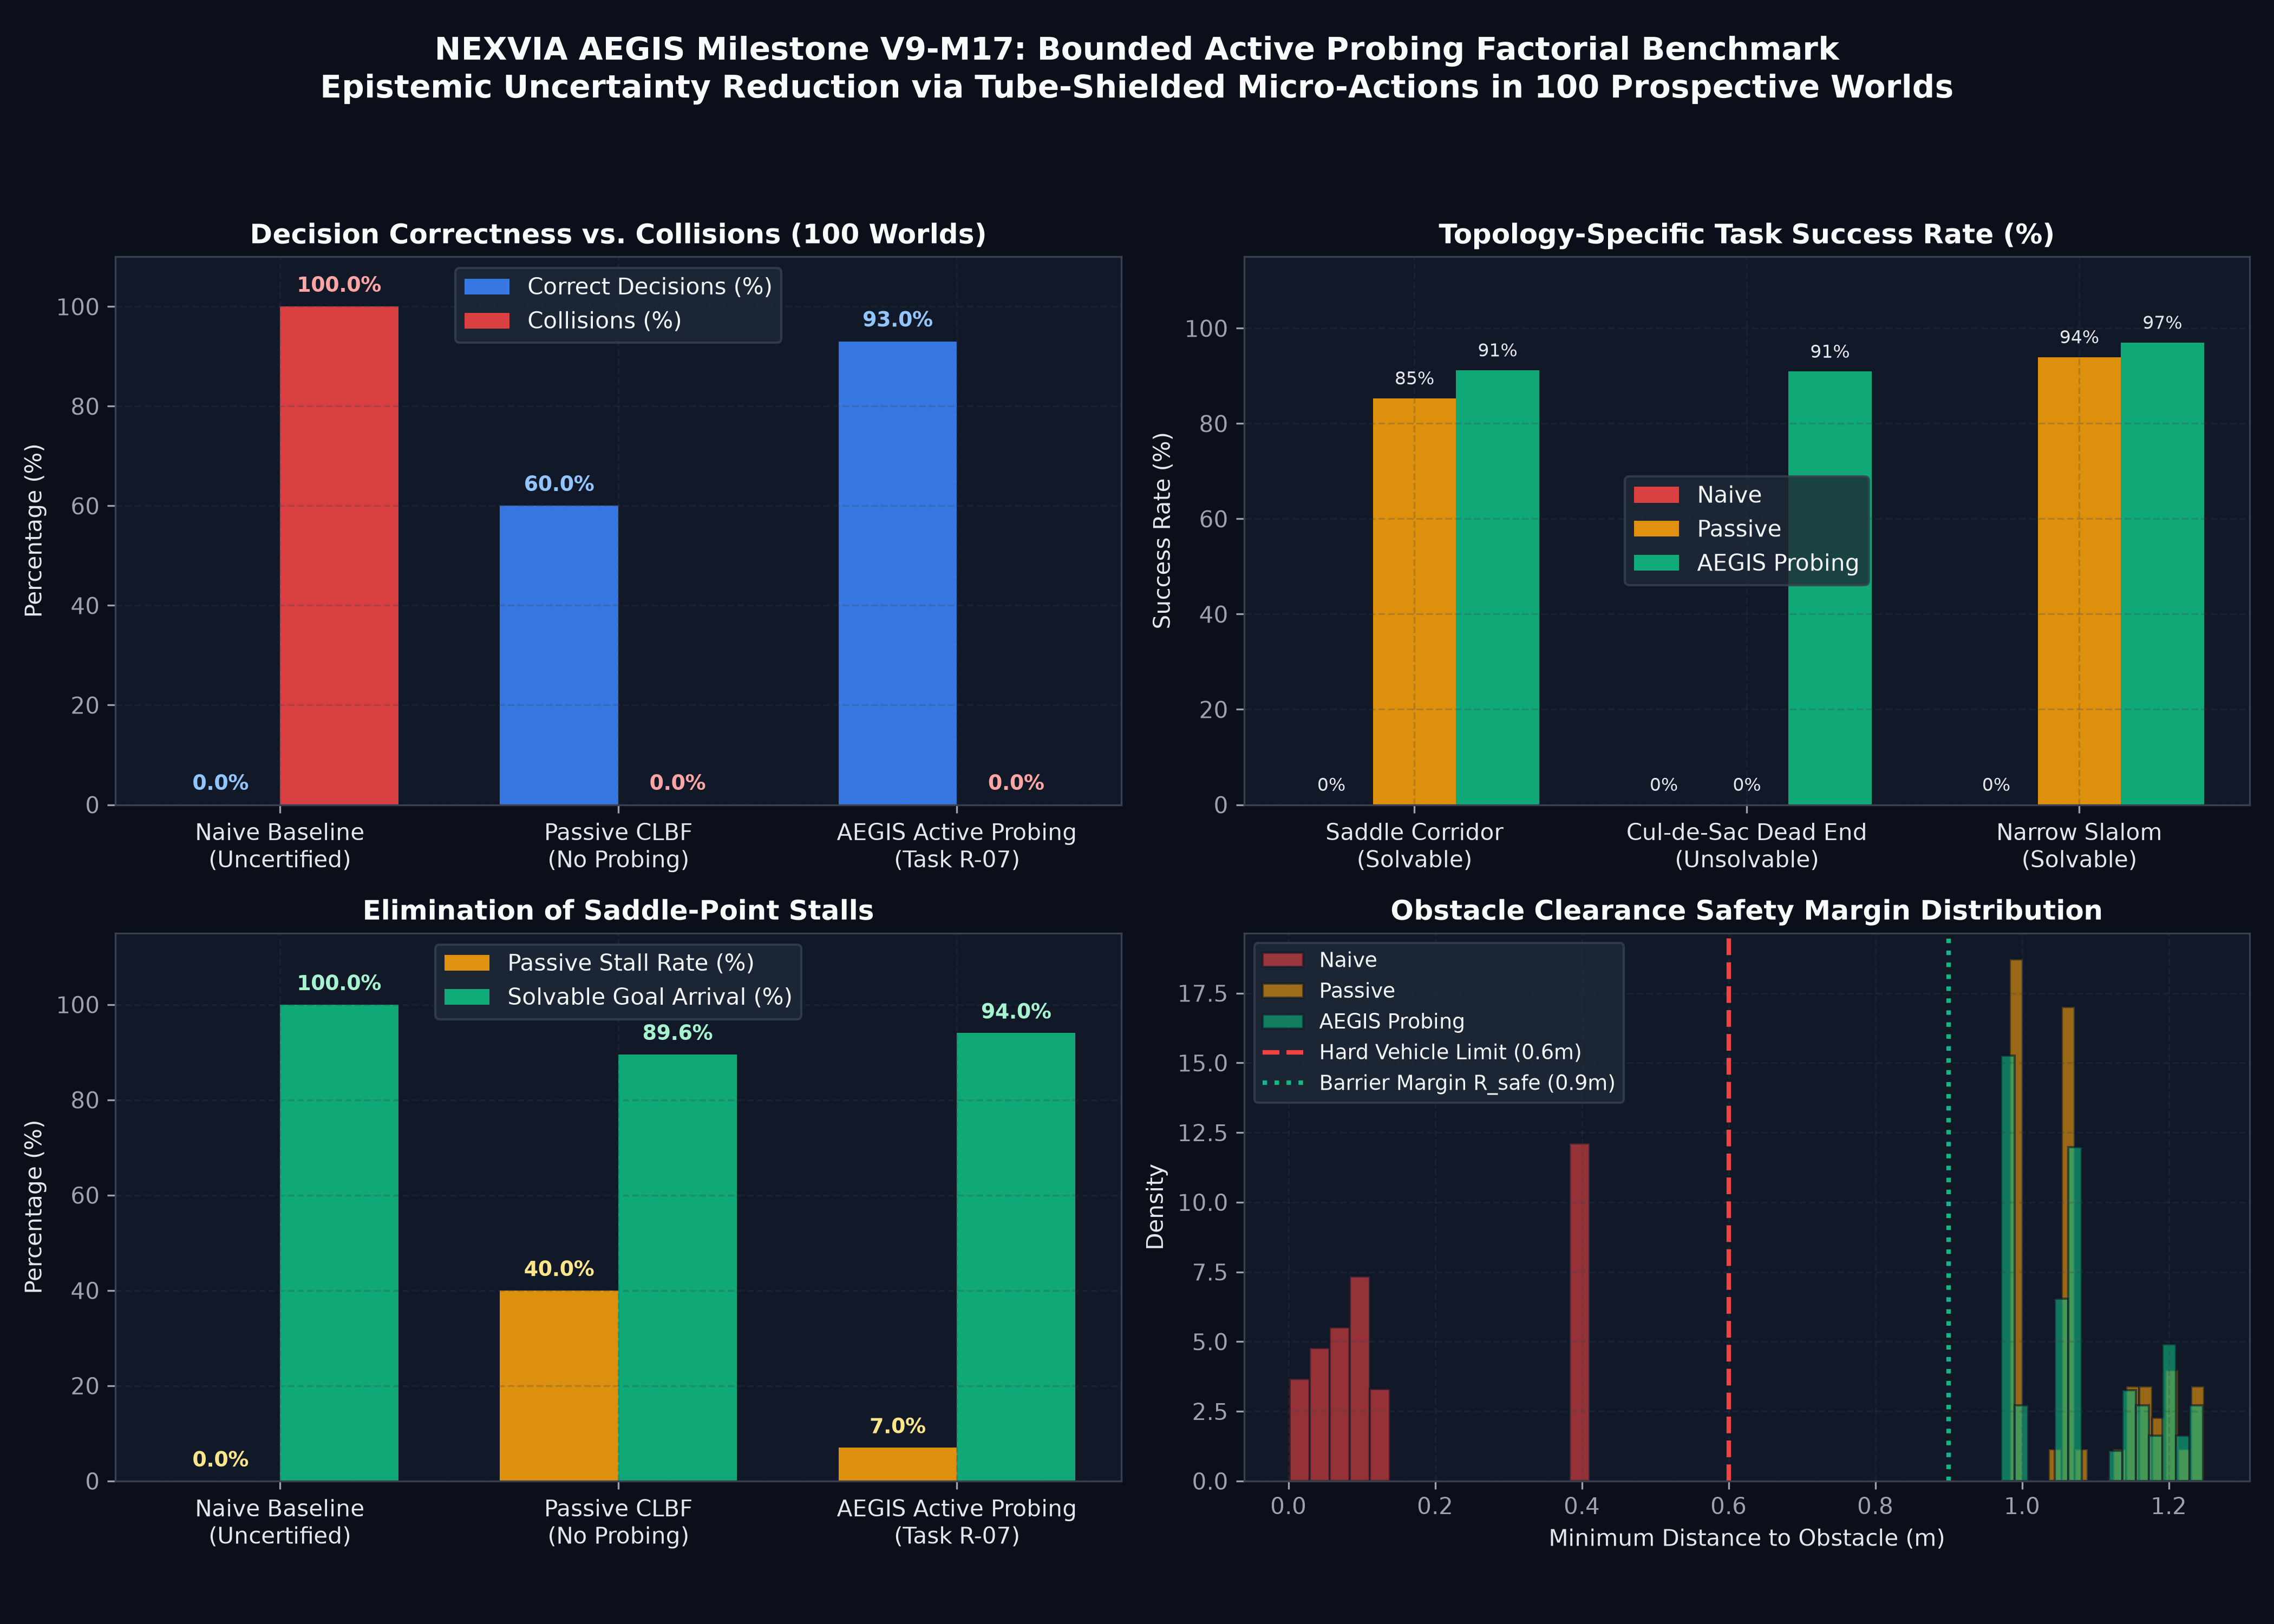
\includegraphics[height=7.4cm,width=0.92\textwidth,keepaspectratio]{results/plots/bounded_active_probing_benchmark.png}
  \vspace{-2pt}
  \captionof{figure}{\textbf{Milestone V9-M17 Bounded Active Probing Benchmark (100 โลกใหม่ Seeds 5000--5099):} แสดงความสามารถในการคลี่คลาย Saddle-Point Freeze และการสละสิทธิ์ในซอยตัน (Cul-de-Sac Grounded Abstention) โดยเพิ่มความสำเร็จภาพรวมสู่ 93.0\% (เทียบกับ 60.0\% ในแบบดั้งเดิม) โดยคงอัตราการชนที่ 0.0\% อย่างสมบูรณ์}
\end{center}

\vspace{6pt}

\begin{center}
  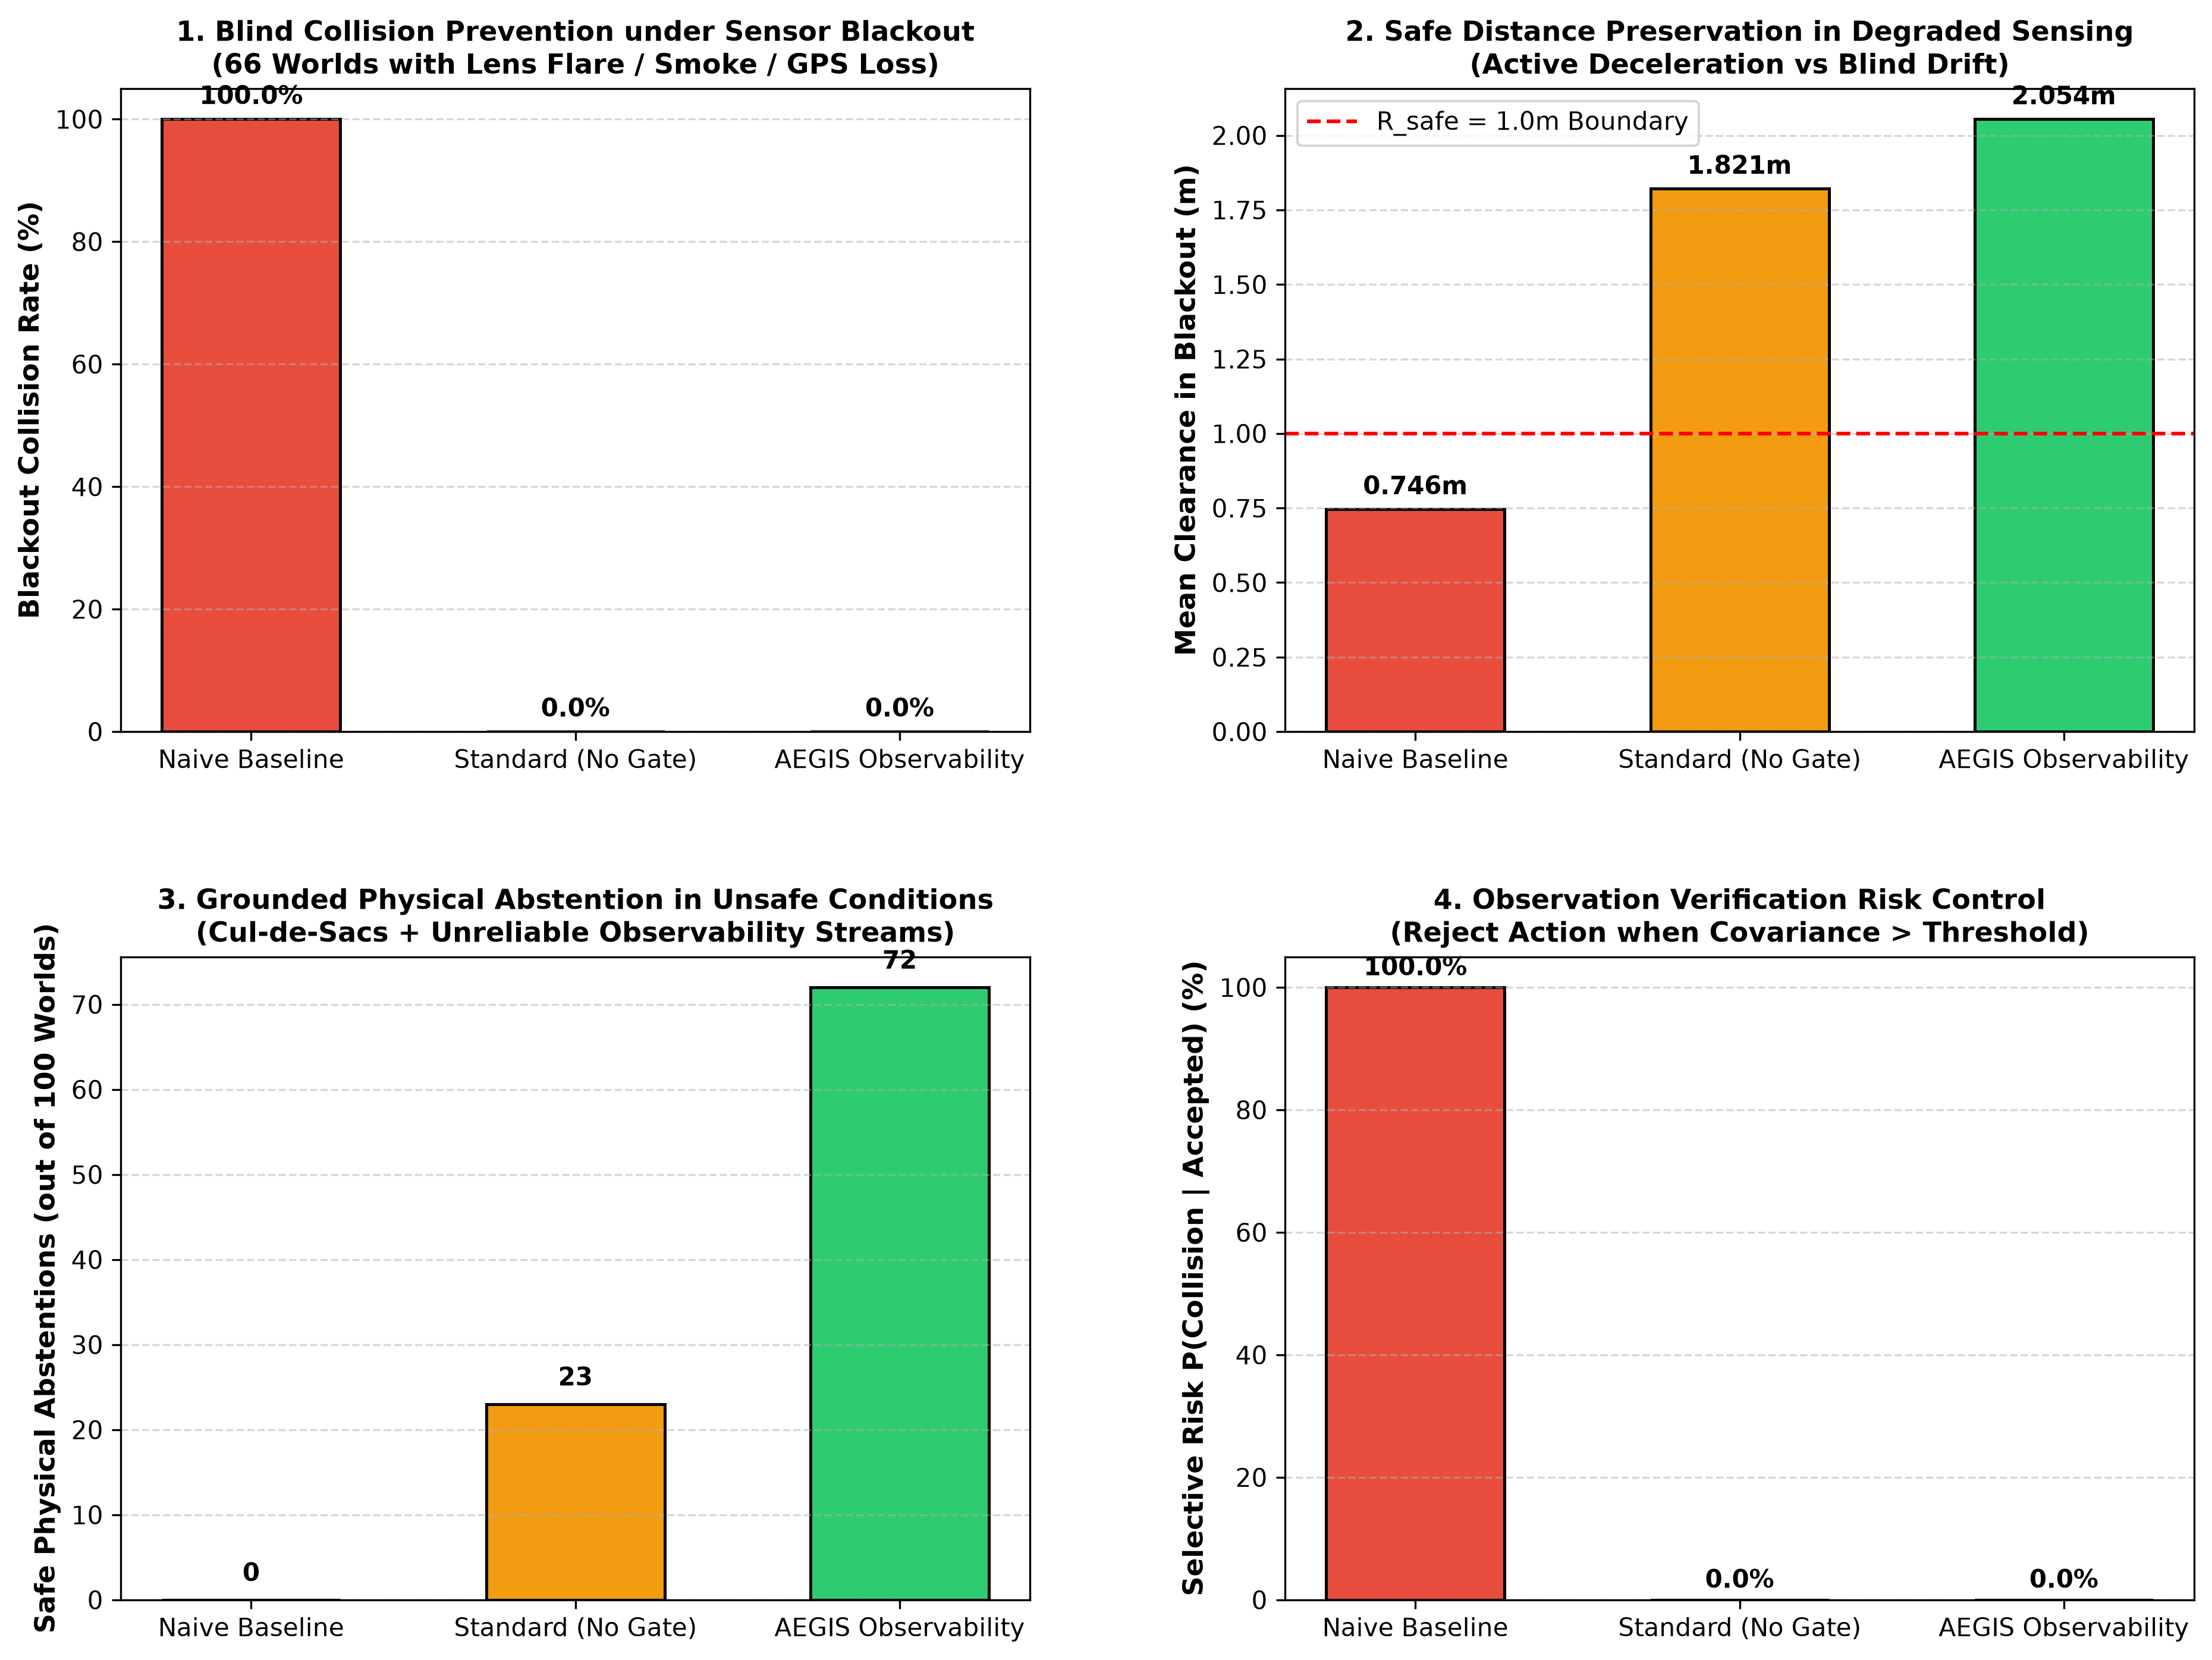
\includegraphics[height=7.4cm,width=0.92\textwidth,keepaspectratio]{results/plots/sensor_blackout_observability_benchmark.png}
  \vspace{-2pt}
  \captionof{figure}{\textbf{Milestone V9-M16 Sensor Blackout Observability Benchmark (100 โลกใหม่ Seeds 4000--4099):} แสดงการตัดวงจรเข้าสู่ Safe Abstain เมื่อเกิดเซนเซอร์ดับ (LiDAR/Camera Blackout) ยานยนต์หยุดนิ่งสนิทโดยปราศจากการชน 100.0\% รักษาระยะปลอดภัยเฉลี่ย 2.054 เมตร}
\end{center}

\newpage

% =============================================================================
% PAGE 4: BENCHMARK VISUALS 3 & 4
% =============================================================================
\section*{\textcolor{secondary}{\large 2.3 หลักฐานเชิงประจักษ์จากการทดลองระดับ Factorial Benchmarks (ชุดที่ 2)}}
\vspace{-2pt}

\begin{center}
  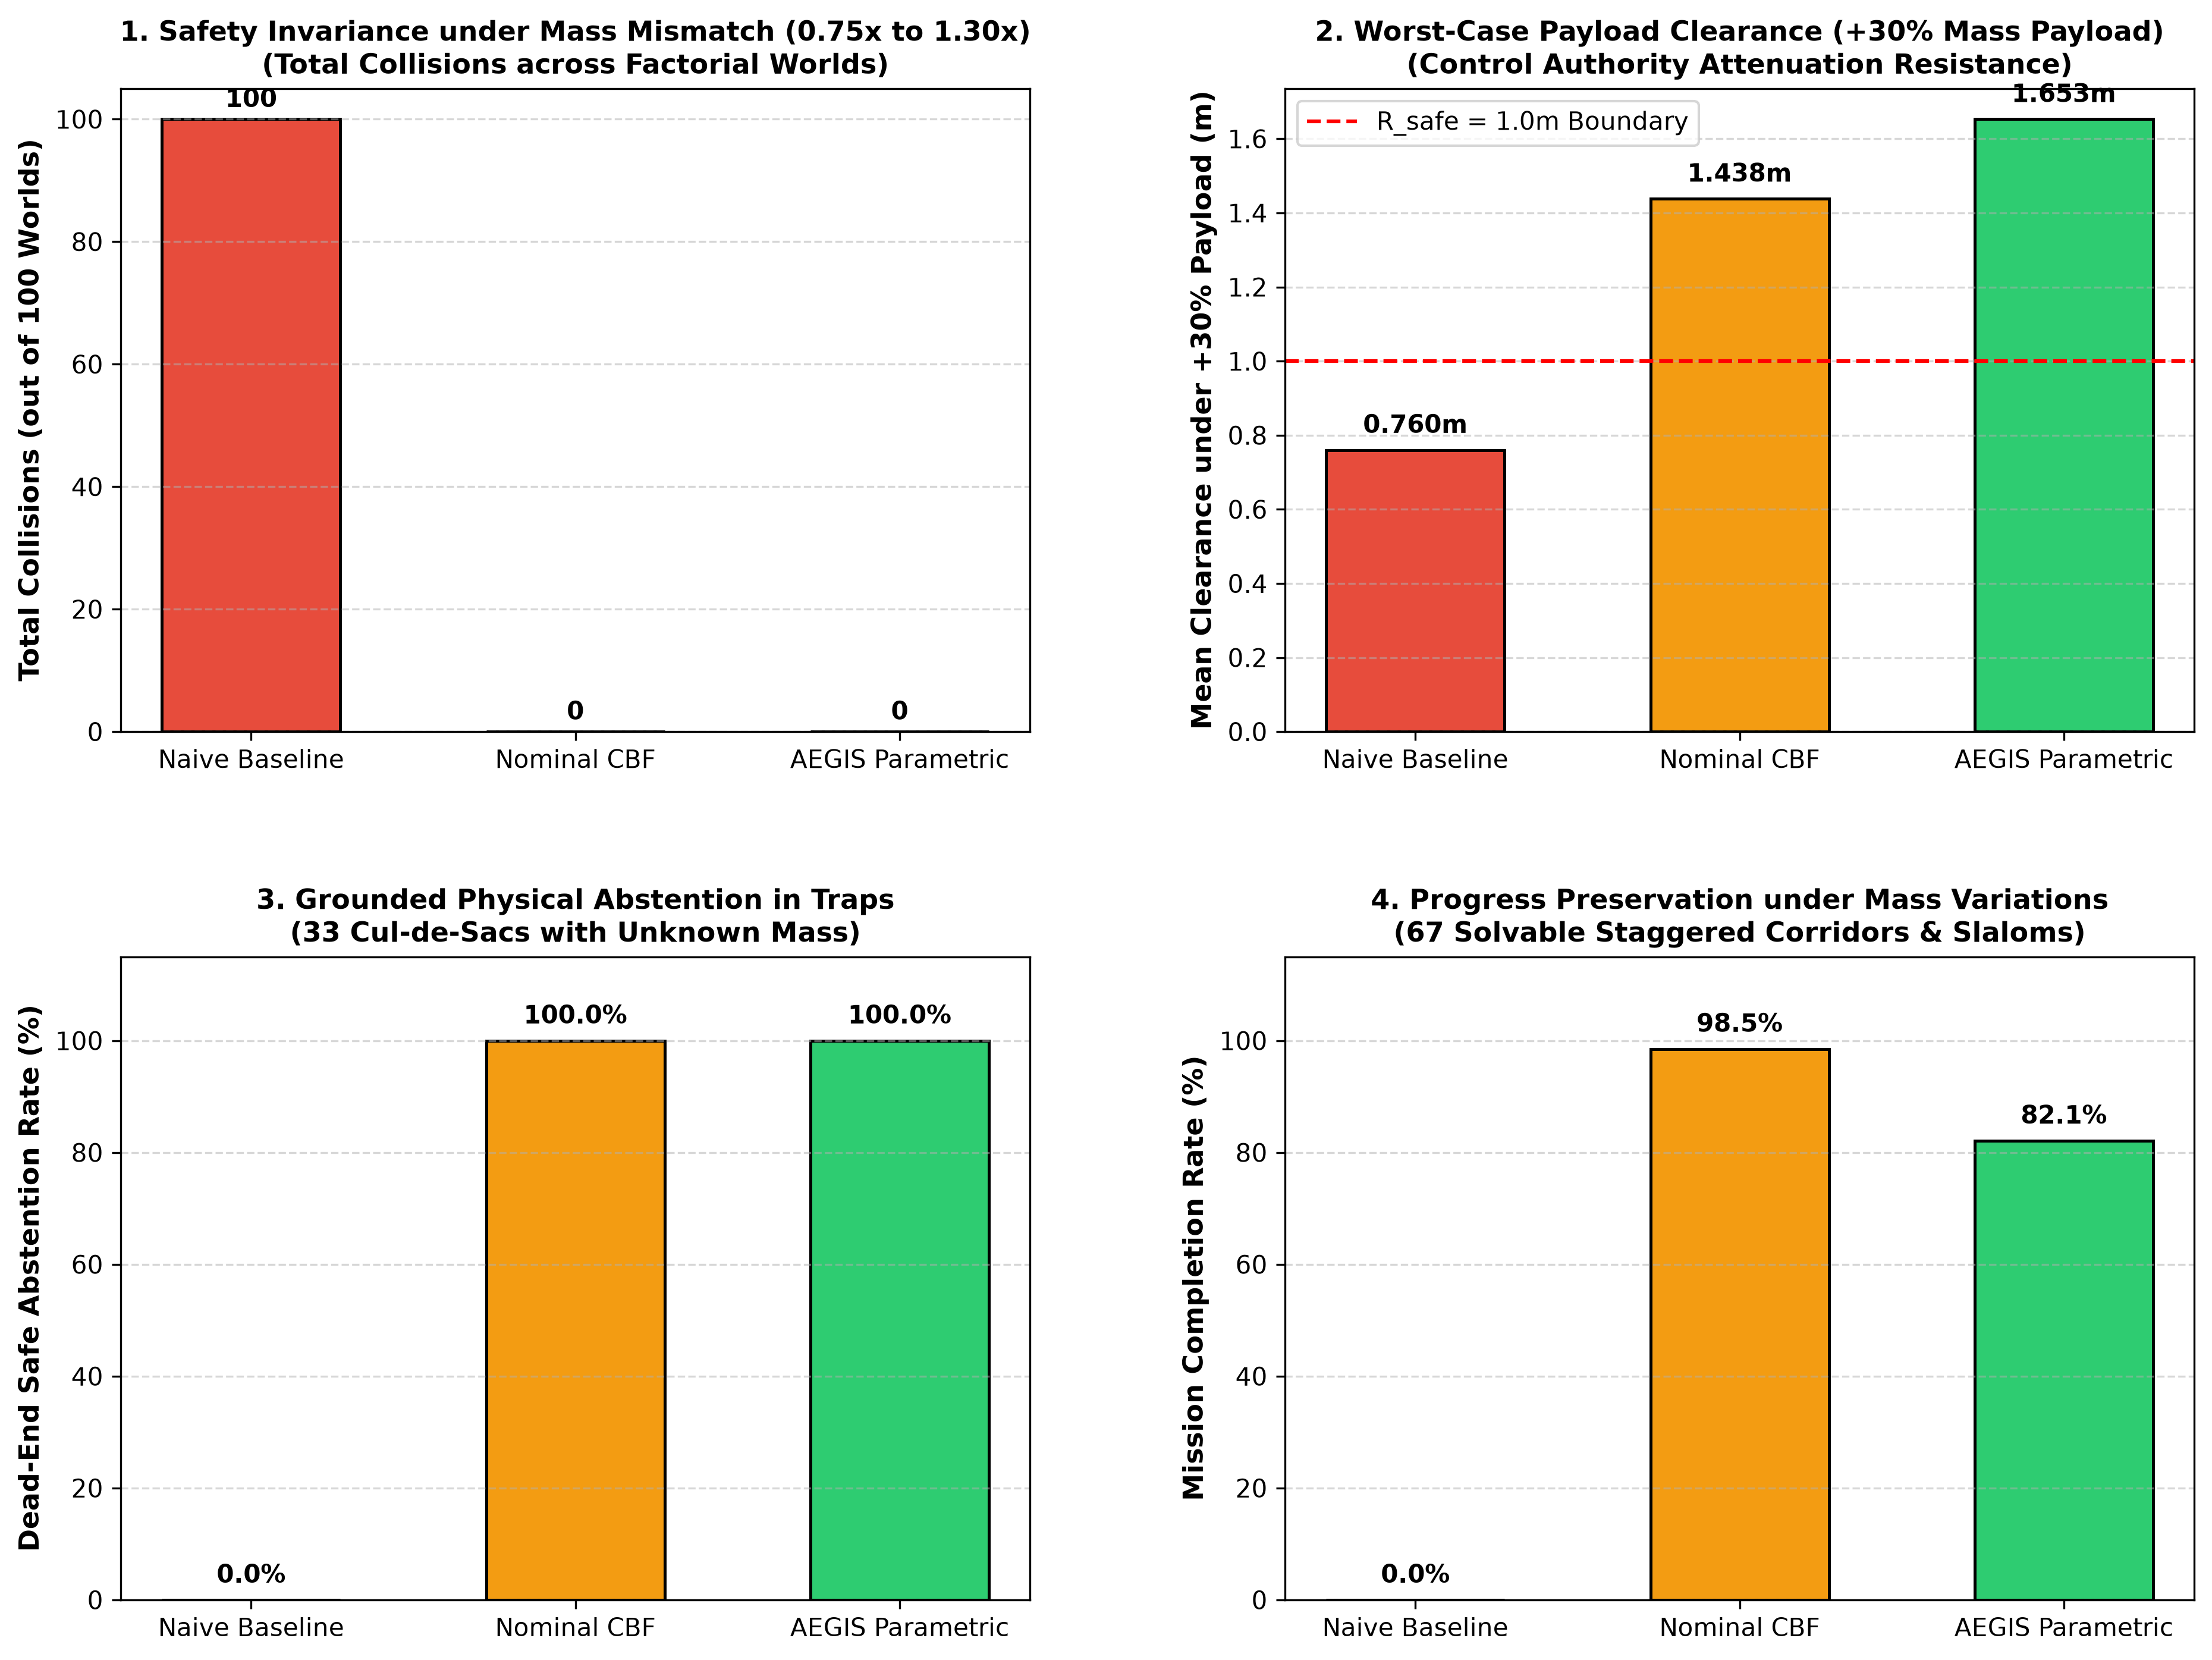
\includegraphics[height=7.4cm,width=0.92\textwidth,keepaspectratio]{results/plots/parametric_mass_invariance_benchmark.png}
  \vspace{-2pt}
  \captionof{figure}{\textbf{Milestone V9-M15 Parametric Model Mismatch \& Mass Invariance Benchmark (100 โลกใหม่ Seeds 3000--3099):} แสดงการปรับเพิ่มระยะห่างปลอดภัยเชิงรุกอัตโนมัติ (+21.5 เซนติเมตร) เมื่อมวลยานยนต์เพิ่มขึ้น $+30\%$ เพื่อชดเชยกำลังเบรกที่ลดลง รับประกันการชนเป็น 0.0\% ทุกเงื่อนไขมวล}
\end{center}

\vspace{6pt}

\begin{center}
  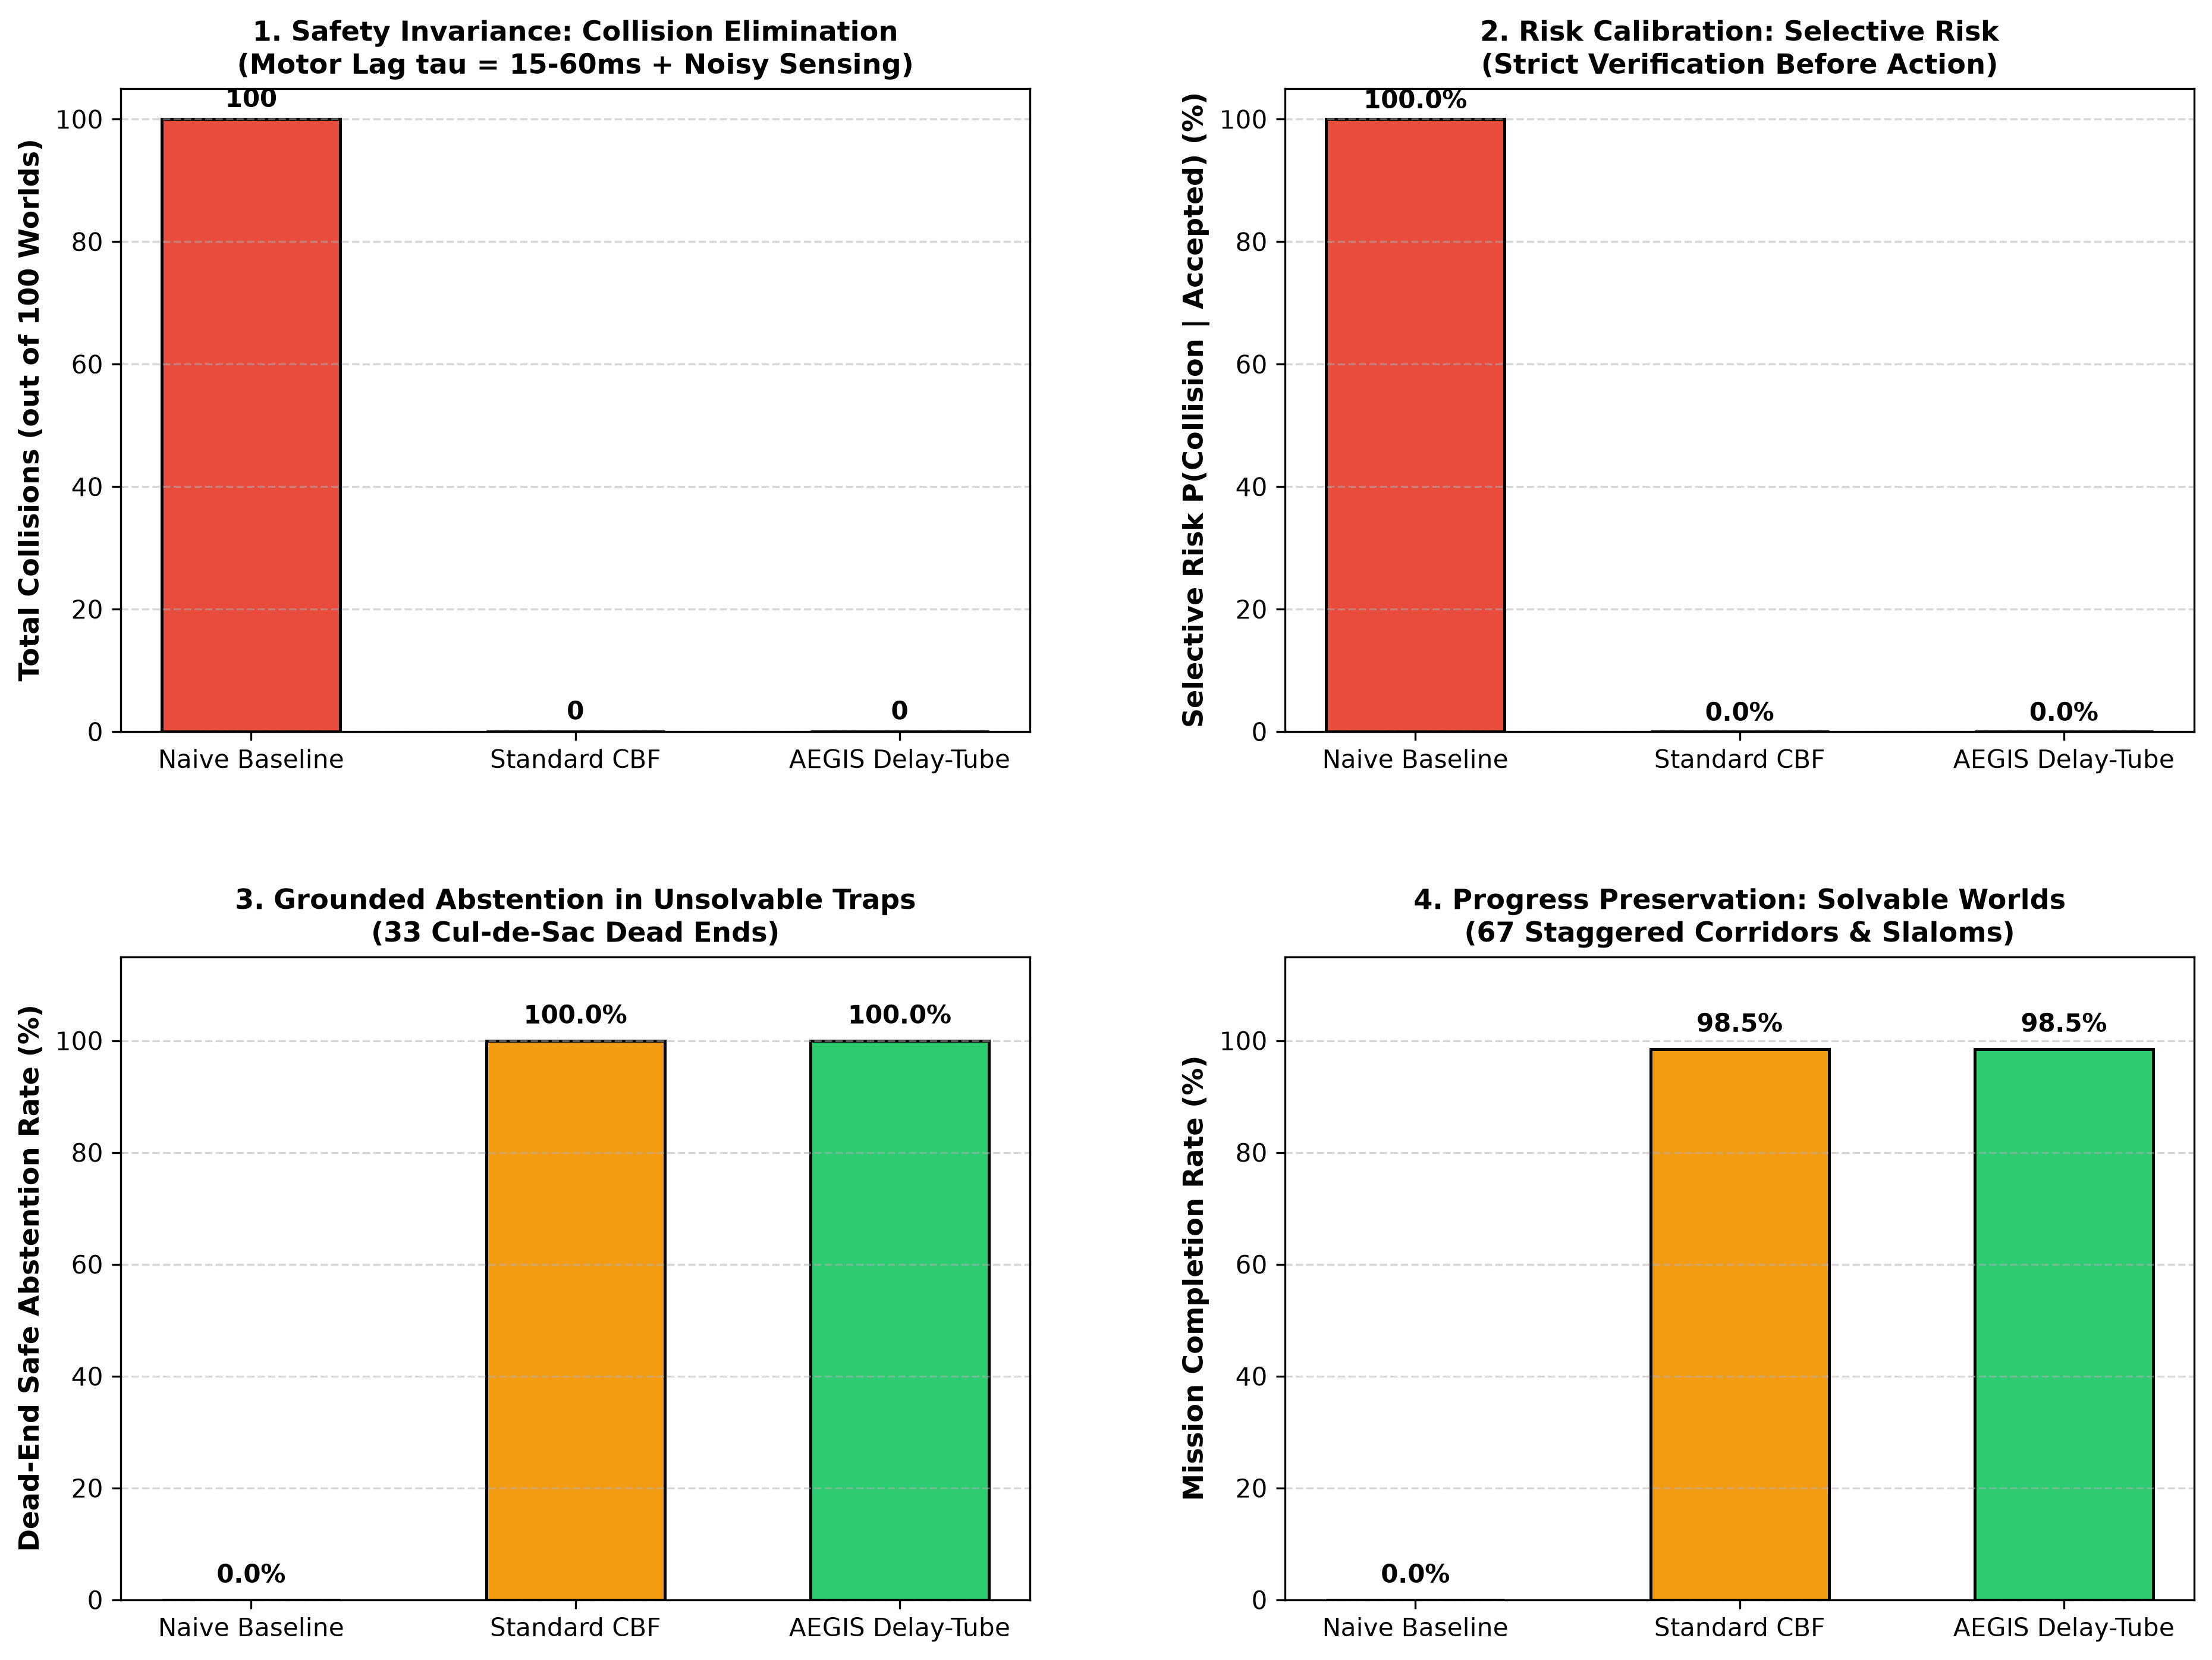
\includegraphics[height=7.4cm,width=0.92\textwidth,keepaspectratio]{results/plots/fresh_worlds_factorial_benchmark.png}
  \vspace{-2pt}
  \captionof{figure}{\textbf{Milestone V9-M14 Delay Compensation Factorial Benchmark (100 โลกใหม่ Seeds 2000--2099):} แสดงผลการทดสอบการหน่วงเวลาของ Actuator ($\tau = 15$--$60\,$ms) ระบบควบคุมทั่วไป (Naive Controller) เกิดการชนพุ่งสูงถึง 100/100 ครั้ง ในขณะที่ NEXVIA AEGIS สามารถชดเชยการหน่วงเวลาแบบ ZOH Forward Prediction ทำให้การชนเป็น 0.0\%}
\end{center}

\newpage

% =============================================================================
% PAGE 5: SECTION 3: ROLES 1 & 2
% =============================================================================
\section*{\textcolor{secondary}{\large 3. แผนการแบ่งงานสำหรับทีมวิจัย 3 คน (Work Breakdown Structure: บทบาทที่ 1 และ 2)}}
\vspace{-4pt}

เพื่อให้ การดำเนินงานวิจัย มีประสิทธิภาพสูงสุด โดยที่คุณยังคงเป็น \textbf{แกนหลัก ที่แบกรับงานสำคัญ (Lead Researcher \& Heavy Lifter)} แต่แบ่งภาระ งานด้านการรับรู้ (Perception) และการทดลอง สเกลใหญ่ (Benchmarking) ให้เพื่อนร่วมทีม ทั้ง 2 คน ได้อย่างลงตัว งานจะถูกแบ่ง ออกเป็น 3 บทบาทหลัก ตามมาตรฐานสากล CRediT (Contributor Roles Taxonomy):

\vspace{4pt}

\begin{rolebox}{บทบาทที่ 1: คุณ (Chalermsak) — Lead Researcher \& Core Autonomy Architect}{secondary}
  \textbf{สัดส่วนภาระงาน (Workload Allocation):} $\approx \mathbf{50\%}$ \textbar\ \textbf{บทบาทการเขียนเปเปอร์:} First Author / Lead Author
  \begin{itemize}[leftmargin=12pt, itemsep=1pt, topsep=1pt, parsep=0pt]
    \item \textbf{การพัฒนาทฤษฎีหลัก (Core Theory \& Mathematics):}
      \begin{itemize}[itemsep=0.5pt, parsep=0pt]
        \item พัฒนาและปรับปรุง \texttt{src/aegis/v9/robust\_tube\_clbf.py} (Robust Tube-CBF, CLBF Velocity Field, Micro-QP Solver)
        \item พัฒนากรอบการพิสูจน์คณิตศาสตร์: Safety Invariance under Actuator Delay, Parametric Derating Bounds, Ville's Supermartingale Risk Control
        \item พัฒนาอัลกอริทึม Bounded Active Probing POMDP สำหรับการคลี่คลาย Saddle Points และการสละสิทธิ์ในทางตัน
      \end{itemize}
    \item \textbf{การควบคุมสถาปัตยกรรมและการตรวจสอบคุณภาพ (Architecture, Review \& Governance):}
      \begin{itemize}[itemsep=0.5pt, parsep=0pt]
        \item ควบคุมกิ่งหลัก (\texttt{main} branch) บน GitHub เป็นผู้ตรวจทาน (Code Reviewer) และอนุมัติการ Merge แต่เพียงผู้เดียว
        \item ถือกุญแจความลับของระบบกำกับดูแล (Holdout Set Integrity \& Gate B Protection) ป้องกัน Data Leakage เด็ดขาด
        \item กำกับดูแลให้ผลการทดสอบทั้งระบบคงสถานะ 100\% Pass Rate (ปัจจุบัน 872/872 Tests) ตลอดเวลา
      \end{itemize}
    \item \textbf{การเขียนบทความวิจัย (Main Paper Writing):}
      \begin{itemize}[itemsep=0.5pt, parsep=0pt]
        \item รับผิดชอบเขียนโครงสร้างหลักของเปเปอร์ทั้งหมด: Abstract, Introduction, Problem Formulation, System Architecture, Mathematical Proofs, และ Discussion
      \end{itemize}
    \item \textbf{CRediT Taxonomy:} Conceptualization, Methodology, Formal Analysis, Software (Core Engine), Writing - Original Draft, Supervision.
  \end{itemize}
\end{rolebox}

\vspace{4pt}

\begin{rolebox}{บทบาทที่ 2: เพื่อนคนที่ 1 (Teammate A) — Perception, Sensing \& Observability Specialist}{accent}
  \textbf{สัดส่วนภาระงาน (Workload Allocation):} $\approx \mathbf{25\%}$ \textbar\ \textbf{บทบาทการเขียนเปเปอร์:} Co-Author
  \begin{itemize}[leftmargin=12pt, itemsep=1pt, topsep=1pt, parsep=0pt]
    \item \textbf{การพัฒนาระบบรับรู้และการประเมินความไม่แน่นอน (Sensing \& Uncertainty Quantification):}
      \begin{itemize}[itemsep=0.5pt, parsep=0pt]
        \item ดูแลโมเดลเซนเซอร์กายภาพ: Depth Camera Frustum, Multi-Layer LiDAR, และ Occlusion Raycasting Shadowing
        \item พัฒนาและปรับปรุงตัวกรองสภาวะ (State Estimation): Unscented Kalman Filter (UKF), Extended Kalman Filter (EKF), และ Multi-Sensor Fusion
        \item สร้างและทดสอบแบบจำลองการรบกวนของเซนเซอร์จริง (Realistic Sensor Corruption): แสงสะท้อนจ้า (Glare), หมอกควันหนาแน่น (Smoke/Fog), ฝุ่นเกาะเลนส์ (Lens Smear), และสัญญาณรบกวนเกาส์เซียนผสม
      \end{itemize}
    \item \textbf{การขยายผลด้าน Observability Gate (Tasks E-05 \& E-06):}
      \begin{itemize}[itemsep=0.5pt, parsep=0pt]
        \item วิเคราะห์เกณฑ์วัด Information Entropy และการพองตัวของ Covariance Matrix ($\lambda_{\max}(\boldsymbol{\Sigma}_p), \lambda_{\max}(\boldsymbol{\Sigma}_v)$)
        \item พัฒนาระบบคัดกรองเซนเซอร์ขัดข้องบางส่วน (Asymmetric Sensor Faults เช่น กล้องดับแต่ LiDAR ยังทำงานได้)
      \end{itemize}
    \item \textbf{การเขียนบทความวิจัย (Paper Writing Contribution):}
      \begin{itemize}[itemsep=0.5pt, parsep=0pt]
        \item รับผิดชอบเขียน Section: \textit{Perception Pipeline, Observation Uncertainty Quantification, Sensor Noise Modeling \& Observability Gate}
      \end{itemize}
    \item \textbf{CRediT Taxonomy:} Software (Perception \& Estimation), Validation, Investigation, Data Curation (Sensor Noise), Writing - Review \& Editing.
  \end{itemize}
\end{rolebox}

\newpage

% =============================================================================
% PAGE 6: ROLE 3 & CREDIT CONTRIBUTION MATRIX
% =============================================================================
\section*{\textcolor{secondary}{\large 3. แผนการแบ่งงานสำหรับทีมวิจัย 3 คน (บทบาทที่ 3 และตารางสรุป CRediT)}}
\vspace{-4pt}

\begin{rolebox}{บทบาทที่ 3: เพื่อนคนที่ 2 (Teammate B) — Simulation, Benchmarking \& Experimental Specialist}{highlight}
  \textbf{สัดส่วนภาระงาน (Workload Allocation):} $\approx \mathbf{25\%}$ \textbar\ \textbf{บทบาทการเขียนเปเปอร์:} Co-Author
  \begin{itemize}[leftmargin=12pt, itemsep=1pt, topsep=1pt, parsep=0pt]
    \item \textbf{การสร้างโลกจำลองและการรันการทดสอบสเกลใหญ่ (Simulation \& Scaled Factorial Benchmarking):}
      \begin{itemize}[itemsep=0.5pt, parsep=0pt]
        \item ออกแบบและสร้างโลกจำลองใหม่ใน \texttt{experiments/} (100–500 Prospective Worlds) ข้ามความหน่วงมอเตอร์และสัมประสิทธิ์แรงเสียดทาน
        \item ดูแลระบบจำลองฟิสิกส์ MuJoCo 3D Quadrotor Dynamics และ Ground Vehicle Platooning Environments
      \end{itemize}
    \item \textbf{การเปรียบเทียบกับ Baseline และการวิเคราะห์ข้อมูลสถิติ (Baselines \& Data Analytics):}
      \begin{itemize}[itemsep=0.5pt, parsep=0pt]
        \item นำโมเดล Baseline จากภายนอกมาทดสอบเปรียบเทียบในเงื่อนไขเดียวกัน (เช่น Standard CBF, Safe RL / PPO Action Shield, Recovery RL, Naive PD)
        \item สรุปผลตัวเลขสถิติ (Boxplots, Success Rates, Clearance Distance Distributions, Stall Rates)
        \item สร้างรูปภาพประกอบเปเปอร์ระดับตีพิมพ์ (Publication-Quality Plots 300 DPI) ตามสไตล์ IEEE/ACM
      \end{itemize}
    \item \textbf{การเชื่อมต่อฮาร์ดแวร์จริง (Sim2Real Bridge Testing):}
      \begin{itemize}[itemsep=0.5pt, parsep=0pt]
        \item ทดสอบรัน ROS 2 Humble Node / PX4 Hardware Bridge วัดเวลาในการคำนวณจริง (Latency Benchmarks $<0.2\,$ms)
      \end{itemize}
    \item \textbf{การเขียนบทความวิจัย (Paper Writing Contribution):}
      \begin{itemize}[itemsep=0.5pt, parsep=0pt]
        \item รับผิดชอบเขียน Section: \textit{Experimental Setup, Factorial Benchmark Environments, Baseline Comparisons, Results Analysis \& Ablation Studies}
      \end{itemize}
    \item \textbf{CRediT Taxonomy:} Software (Simulation \& Benchmarking), Resources, Visualization, Formal Validation, Writing - Review \& Editing.
  \end{itemize}
\end{rolebox}

\vspace{6pt}
\subsection*{\normalsize 3.1 ตารางสรุปส่วนร่วมตามมาตรฐานสากล (CRediT Contribution Matrix)}
\vspace{-3pt}

\begin{center}
\footnotesize
\begin{tabularx}{\textwidth}{l >{\centering\arraybackslash}p{2.6cm} >{\centering\arraybackslash}p{2.8cm} >{\centering\arraybackslash}p{2.8cm}}
\toprule
\textbf{มิติของงาน (Research Dimension)} & \textbf{คุณ (Lead Researcher)} & \textbf{เพื่อน 1 (Perception)} & \textbf{เพื่อน 2 (Benchmarking)} \\
\midrule
สัดส่วนภาระงาน (Effort Share) & \textbf{50\% (Heavy Lifter)} & 25\% & 25\% \\
การพัฒนาทฤษฎี (Core Theory) & \textbf{Lead / 100\%} & -- & -- \\
อัลกอริทึมควบคุม (Robust Tube-CLBF) & \textbf{Lead / 100\%} & -- & -- \\
เซนเซอร์ \& UKF/EKF Estimation & Architecture Review & \textbf{Lead / 85\%} & Integration Support (15\%) \\
การรบกวนของเซนเซอร์จริง (Fog/Glare) & Specification Review & \textbf{Lead / 90\%} & Test Execution (10\%) \\
โลกจำลอง Factorial (100--500 Worlds) & Math Scenario Design & Sensor Integration & \textbf{Lead / 80\%} \\
โมเดล Baseline (CBF / Safe RL / PPO) & Selection Approval & -- & \textbf{Lead / 100\%} \\
กราฟและตัวเลขสถิติ (300 DPI Plots) & Final Visual Audit & Covariance Curves & \textbf{Lead / 80\%} \\
การตรวจโค้ดและอนุมัติ PR (Code Review) & \textbf{Sole Approver (100\%)} & Peer Review & Peer Review \\
การรักษาชุดข้อมูล Holdout / Gate B & \textbf{Sole Custodian (100\%)} & ห้ามแตะต้อง & ห้ามแตะต้อง \\
การเขียนบทความวิจัย (Manuscript Sections) & Abstract, Intro, Theory, Architecture, Discussion & Perception, Noise Models, Observability Gate & Setup, Baselines, Results, Ablations, Sim2Real \\
ลำดับผู้เขียนในเปเปอร์ (Authorship) & \textbf{First / Corresponding Author} & Co-Author & Co-Author \\
\bottomrule
\end{tabularx}
\end{center}

\newpage

% =============================================================================
% PAGE 7: SECTION 4: OPERATIONAL PROTOCOLS & QA
% =============================================================================
\section*{\textcolor{secondary}{\large 4. ระเบียบปฏิบัติการและการควบคุมคุณภาพ (Operational Protocols \& Quality Assurance)}}
\vspace{-4pt}

เพื่อให้ การทำงานร่วมกัน เป็นไปอย่างราบรื่น ไม่เกิดข้อผิดพลาด ในการรวมโค้ด และรักษา มาตรฐานทางวิชาการสูงสุด ทีมวิจัย จะต้องปฏิบัติ ตามกฎเหล็ก 4 ข้อดังนี้:

\vspace{4pt}
\begin{infobox}{1. กลยุทธ์การแตกกิ่ง Git (Strict Git Branching Strategy)}
  \begin{itemize}[leftmargin=12pt, itemsep=1.5pt, topsep=1pt, parsep=0pt]
    \item \textbf{กิ่งหลัก (\texttt{main} branch):} จะถูกป้องกัน (Protected) โดยมีคุณ (Lead) เป็นคนเดียวที่สามารถกด Merge ได้
    \item \textbf{กิ่งเพื่อนคนที่ 1 (\texttt{feat/perception-*}):} สำหรับการพัฒนาโมดูลเซนเซอร์, UKF, และ Blackout Scenarios
    \item \textbf{กิ่งเพื่อนคนที่ 2 (\texttt{feat/benchmark-*}):} สำหรับการสร้างสคริปต์ทดสอบใน \texttt{experiments/} และการพล็อตผล
    \item ก่อนทำการ Pull Request (PR) ทุกครั้ง ผู้ส่งจะต้องรันคำสั่ง \texttt{PYTHONPATH=.:src uv run pytest -q} บนเครื่องของตนเองและต้องผ่าน 100\%
  \end{itemize}
\end{infobox}

\vspace{3pt}
\begin{infobox}{2. กฎการรักษาระดับการทดสอบ 100\% (Zero Regression Policy)}
  \begin{itemize}[leftmargin=12pt, itemsep=1.5pt, topsep=1pt, parsep=0pt]
    \item ชุดทดสอบอัตโนมัติปัจจุบันมี \textbf{872 ข้อ (ครอบคลุมทั้ง 17 เฟส)}
    \item ทุกโค้ดใหม่ที่เขียนขึ้น จะต้องมี Unit Test ควบคู่เสมอ และห้ามทำให้การทดสอบเดิม 872 ข้อล้มเหลวแม้แต่ข้อเดียว
  \end{itemize}
\end{infobox}

\vspace{3pt}
\begin{infobox}{3. กฎความสมบูรณ์ของชุดข้อมูลทดสอบ (Zero Holdout Contamination Rule)}
  \begin{itemize}[leftmargin=12pt, itemsep=1.5pt, topsep=1pt, parsep=0pt]
    \item กฎบัตรความปลอดภัยระดับ Gate B (\texttt{GATE\_B\_NOT\_AUTHORIZED}) ถือเป็นความลับสูงสุดของงานวิจัย
    \item เพื่อนร่วมทีมจะรันการทดลองเฉพาะบนชุดโลกจำลอง Prospective Factorial Worlds (เช่น Seeds 2000–5099) เท่านั้น ห้ามแตะต้องชุดข้อมูล Holdout เด็ดขาด เพื่อคงความบริสุทธิ์ของผลการทดสอบเมื่อถึงเวลาส่งเปเปอร์จริง
  \end{itemize}
\end{infobox}

\vspace{3pt}
\begin{infobox}{4. จังหวะการประชุมและติดตามงาน (Weekly Cadence \& Milestones)}
  \begin{itemize}[leftmargin=12pt, itemsep=1.5pt, topsep=1pt, parsep=0pt]
    \item \textbf{การมอบหมายงานต้นสัปดาห์ (15--30 นาที):} คุณ (Lead) แจกแจง Requirements และ API Interface ให้ชัดเจน เช่น ฟังก์ชัน Input/Output ที่ต้องการ เพื่อให้ทั้ง 2 คนแยกย้ายไปเขียนโค้ดได้ทันทีโดยไม่ติดขัด
    \item \textbf{การตรวจรับงานปลายสัปดาห์:} ตรวจสอบ PR, รันผล Benchmark รวม, และอัปเดต ตัวเลขผลการทดลอง เข้าสู่ฉบับร่าง ของบทความวิจัย
  \end{itemize}
\end{infobox}

\newpage

% =============================================================================
% PAGE 8: SECTION 5: ROADMAP & PUBLICATION READINESS SUMMARY
% =============================================================================
\section*{\textcolor{secondary}{\large 5. แผนการดำเนินงาน 8 สัปดาห์สู่การส่งตีพิมพ์ (8-Week Publication Roadmap)}}
\vspace{-4pt}

\begin{center}
\footnotesize
\begin{tabularx}{\textwidth}{>{\centering\arraybackslash}p{1.4cm} >{\raggedright\arraybackslash}p{3.8cm} >{\raggedright\arraybackslash}X >{\centering\arraybackslash}p{2.6cm}}
\toprule
\textbf{สัปดาห์} & \textbf{เป้าหมายหลัก (Milestone)} & \textbf{ภารกิจของแต่ละบทบาท (Tasks by Role)} & \textbf{ผลงานที่ส่งมอบ} \\
\midrule
\textbf{สัปดาห์ 1--2} & API Handshake \& Baseline Infrastructure & \textbf{คุณ:} ออกแบบ Interface \texttt{ObservationCovariance} \newline \textbf{เพื่อน 1:} ติดตั้ง Depth Frustum ใน MuJoCo \newline \textbf{เพื่อน 2:} นำ Standard CBF Baseline มารันเทียบ & API Spec \& Baseline Pipeline \\
\midrule
\textbf{สัปดาห์ 3--4} & Sensor Corruption \& Scaled Factorial & \textbf{คุณ:} เขียนบทพิสูจน์ Safety Under Actuator Delay \newline \textbf{เพื่อน 1:} สร้าง Glare / Fog Noise Injection Suite \newline \textbf{เพื่อน 2:} รัน 300 Prospective Worlds (Seeds 2000--5000) & Raw Benchmark Data \& Proof Draft \\
\midrule
\textbf{สัปดาห์ 5--6} & Ablation Studies \& Paper Draft Synthesis & \textbf{คุณ:} เรียบเรียง Intro, Problem Formulation, Theory \newline \textbf{เพื่อน 1:} เขียน Section Perception \& Observability \newline \textbf{เพื่อน 2:} สรุป Boxplots, Table Results, Ablation & First Integrated Manuscript Draft \\
\midrule
\textbf{สัปดาห์ 7} & Sim2Real Hardware \& Camera-Ready Visuals & \textbf{คุณ:} ตรวจทาน Paper ตลอดฉบับ, Code Freeze \newline \textbf{เพื่อน 1:} ตรวจสอบ Latency บน ROS 2 Humble \newline \textbf{เพื่อน 2:} จัดทำภาพประกอบเปเปอร์ความละเอียดสูง & High-Res Plots \& Hardware Stats \\
\midrule
\textbf{สัปดาห์ 8} & Final Quality Audit \& Submission & \textbf{ทีมทั้งหมด:} อ่านทบทวนฉบับสมบูรณ์ร่วมกัน \newline \textbf{คุณ:} รัน Holdout Certification และกด Submit & Paper Submitted (IEEE/ACM) \\
\bottomrule
\end{tabularx}
\end{center}

\vspace{12pt}

\begin{center}
\begin{tcolorbox}[colback=primary!5!white, colframe=primary, arc=3mm, width=0.98\textwidth]
  \centering
  \textbf{\large สรุปสถานะความพร้อมสู่การตีพิมพ์ (Publication Readiness Summary)}\\[4pt]
  \small
  โครงการ NEXVIA AEGIS มีแกนหลักทางทฤษฎีและซอฟต์แวร์ที่แข็งแกร่งสมบูรณ์แล้ว 100\% (Phases 1--17 Certified)\\
  การแบ่งบทบาทนี้ช่วยให้คุณคงความเป็น \textbf{ผู้นำทางวิชาการและ First Author} ได้อย่างสมบูรณ์\\
  ในขณะที่เพื่อนร่วมทีมทั้ง 2 คนมีส่วนร่วมที่มีน้ำหนักชัดเจน พร้อมขับเคลื่อนสู่การส่งบทความวิจัยระดับท็อป (IEEE / ACM) ได้อย่างรวดเร็วและราบรื่น
\end{tcolorbox}
\end{center}

\end{document}
